De lo que este algoritmo trata es de marcar todos los vértices como no utilizados. El algoritmo parte
de un vértice origen que será ingresado, a partir de ese vértices evaluaremos sus adyacentes, como
dijkstra usa una técnica greedy - La técnica greedy utiliza el principio de que para que un camino
sea óptimo, todos los caminos que contiene también deben ser óptimos- entre todos los vértices
adyacentes, buscamos el que esté más cerca de nuestro punto origen, lo tomamos como punto
intermedio y vemos si podemos llegar más rápido a través de este vértice a los demás. Después
escogemos al siguiente más cercano (con las distancias ya actualizadas) y repetimos el proceso.
Esto lo hacemos hasta que el vértice no utilizado más cercano sea nuestro destino. Al proceso
de actualizar las distancias tomando como punto intermedio al nuevo vértice se le conoce como
relajación.

Teniendo un grafo dirigido ponderado de N nodos no aislados, sea x el nodo inicial, un vector D de tamaño N guardará al final del algoritmo las distancias desde x al resto de los nodos.

\begin{enumerate}
	\item Inicializar todas las distancias en D con un valor infinito relativo ya que son desconocidas al principio, exceptuando la de x que se debe colocar en 0 debido a que la distancia de x a x sería 0.
	\item Sea a = x (tomamos a como nodo actual).
	\item Recorremos todos los nodos adyacentes de a, excepto los nodos marcados, llamaremos a estos nodos no marcados v$_{i}$.
	\item  Para el nodo actual, calculamos la distancia tentativa desde dicho nodo a sus 
	vecinos con la siguiente fórmula: dt(v$_{i}$.) = D$_{a}$. + d(a,v$_{i}$.). Es decir, la 
	distancia tentativa del nodo \textquoteleft v$_{i}$.\textquoteright es la distancia que 
	actualmente tiene el nodo en el vector D más la distancia desde dicho el nodo 
	\textquoteleft a\textquoteright (el actual) al nodo v$_{i}$. Si la distancia tentativa 
	es menor que la distancia almacenada en el vector, actualizamos el vector con esta 
	distancia tentativa. Es decir: Si dt(v$_{i}$) $\textless$ D$_{vi}$ $\rightarrow$ D$_{vi}$ = dt(v$_{i}$)
	\item Marcamos como completo el nodo a.
	\item Tomamos como próximo nodo actual el de menor valor en D (puede hacerse almacenando los valores en una cola de prioridad) y volvemos al paso 3 mientras existan nodos no marcados.
\end{enumerate}



Una vez terminado al algoritmo, D estará completamente lleno.

\begin{figure}[h]
	\centering 
	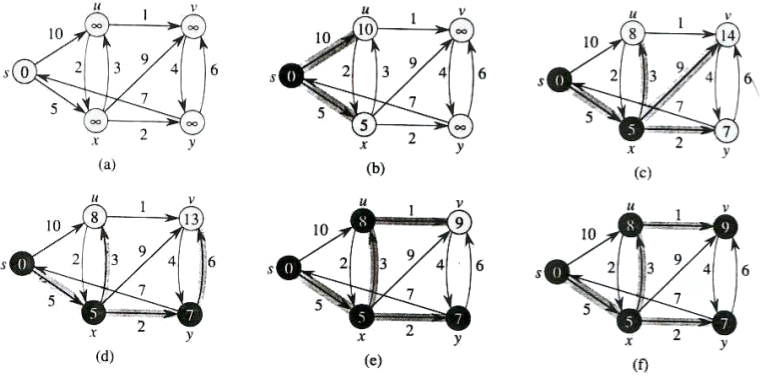
\includegraphics[scale=0.55]{img/algoritmo_dijkstra}
	\caption{Ejecucción del algoritmo Dijkstra comenzando por el nodo {\em s}.}
	\label{contexto:figura}
\end{figure}